\section{Implementation}\label{sec:implementation}

Once all the requirements of the system were laid down, the implementation phase could commence. In the following chapter the implementation of selected Use cases and requirements is described. The system is implemented as two separate segments: Authentication -- exposing the FIDO2 flow and the use of an authenticator, and Authorisation -- demonstrating the OAuth flow.  

\subsection{Authentication}\label{sec:implementation-authentication}
In this section we describe, how the authentication flows are implemented in the prototype. Following the findings from the Analysis and Design chapters, we proceed to implement the sign-in use case, where the user uses their authenticator to sign-in to a service (UC-1), and the registration use case, where a new authenticator is added to user's account (UC-5). The sign-in use case in the prototype omits the use of \acrshort{jwt} for authentication, and only considers the use of a \acrshort{fido} key.

\subsubsection{Setup}
Essentially, the prototype demonstrates the communication between a user agent and the \acrshort{aaserver}. A regular internet browser could be used as the user agent, but a custom \acrshort{aaserver} must be implemented to carry out the sign-in and registration activities. While it would be possible to demonstrate this by running a server locally on developer's machine, we have chosen to deploy the \acrshort{aaserver} into the cloud to allow for testing across different platforms. Google Cloud Compute Engine\footnote{\url{https://cloud.google.com/compute/}, accessed 19 May 2019} was arbitrarily chosen to host the \acrshort{aaserver}, due to offering a range of free services, making it suitable for testing. A virtual machine running Debian 9 distribution of Linux as the operating system was created in the cloud, and Apache Tomcat 9\footnote{\url{http://tomcat.apache.org/}, accessed 19 May 2019} was installed as the primary host of web server code. The combination of Linux and Tomcat was chosen to support serving of dynamic web content via Java Servlet technology. Java was chosen as the server-side language, due to its wide-spread use and existing FIDO libraries and examples.

The server was configured to accept connections from any IP address over the port \texttt{433} on the \texttt{/AAFidoServer} endpoint. A self-signed certificate was deployed at the server and the server was configured to enforce the use of \texttt{HTTPS} for any requests to the endpoint. This was due to the fact, that any manipulation with user credentials (such as FIDO key) in the user agent must be made via \textit{secure context}\footnote{\url{https://www.w3.org/TR/secure-contexts/}, accessed 19 May 2019}, which mandates the use of encryption when serving a web page.

A domain name \texttt{fidoserver.ml} was registered on a cost-free top-level domain\footnote{\url{https://www.freenom.com/en/index.html?lang=en}, accessed 19 May 2019} and the responsible \acrshort{dns} server was configured to direct requests to the public IP address of the server. This was required by the browser in addition to \texttt{HTTPS} to establish the secure context~\cite{Hodges2012HTTPHSTS}.

A MongoDB database was also deployed on the server to retain user data. The choice of the database was also arbitrary, motivated mainly by ease of use and existing Java integration libraries.

\subsubsection{Libraries used}
Java Servlets are part of Java Enterprise Edition (EE) and provide an interface to easily receive and respond to HTTP requests made to the server. Developer environments designed for Java EE also offer other tools for creating web applications. These were used to create two user-facing pages (one for registration and one for sign-in) and two JavaScript files orchestrating the process in the browser. These were all bound together in a web application (web archive file \texttt{.war}) and deployed on the Apache Tomcat server.

Yubico java-webauthn-server library\footnote{\url{https://github.com/Yubico/java-webauthn-server}, accessed 19 May 2019} 1.2.0 was used at the server side to build and verify Webauthn assertions and attestations. An example Webauthn implementation from Google\footnote{\url{https://github.com/google/webauthndemo}, accessed 19 May 2019} was also used as a model for user-agent scripts, although customisation was needed to adapt the user-agent scripts to assertions built by the Yubico's Webauthn server library.

MongoDB Synchronous Driver\footnote{\url{https://mvnrepository.com/artifact/org.mongodb/mongodb-driver-sync/3.9.0}, accessed 19 May 2019} in version 3.9.0 was used to communicate with the local database. This library contains serialisation and deserialisation features to map Java classes to database objects and vice versa.

\subsubsection{Structure}
The architecture of the authentication part of the prototype loosely follows the \acrlong{movp} architectural pattern. This pattern separates the application into three layers, separating the responsibility of each layer.

The model is responsible for manipulating, updating and maintaining the data in the system~\cite{MRizwan2014APresenter}. In this part of the prototype, the model is represented by four \texttt{store} classes, which describe the structure of the data and four \texttt{connector} classes that manipulate this data.

The presenter captures user input and feeds the data to the model. The presenter also adjusts the view accordingly, based on an event triggered by the user, or when a change is requested by the model~\cite{MRizwan2014APresenter}. Here, the presenter is represented by the JavaScript files that execute in the user agent, four classes, which extend the \texttt{HttpServlet} of Java Servlet library, and which execute on the server and a small number of utility classes of the Webauthn server library that help process and unwrap user input.

Finally, the view is responsible for presenting the user interface and displaying data to the user. The view in this part of the prototype is represented by two Java Server Pages files, which exclusively contain the HTML representation of the user facing part of the prototype.

Class diagram in Figure~\ref{fig:class-diagram} captures the classes of this part of the prototype. These classes, together with the configuration file describing the URL endpoints and their mapping to the \texttt{HttpServlet} classes make up the web application, which is packaged and deployed on the web server.

\newgeometry{left=1cm,right=1cm,top=1cm,bottom=.8cm,footskip=.3cm}
\begin{sidewaysfigure}[p]
    \centering
    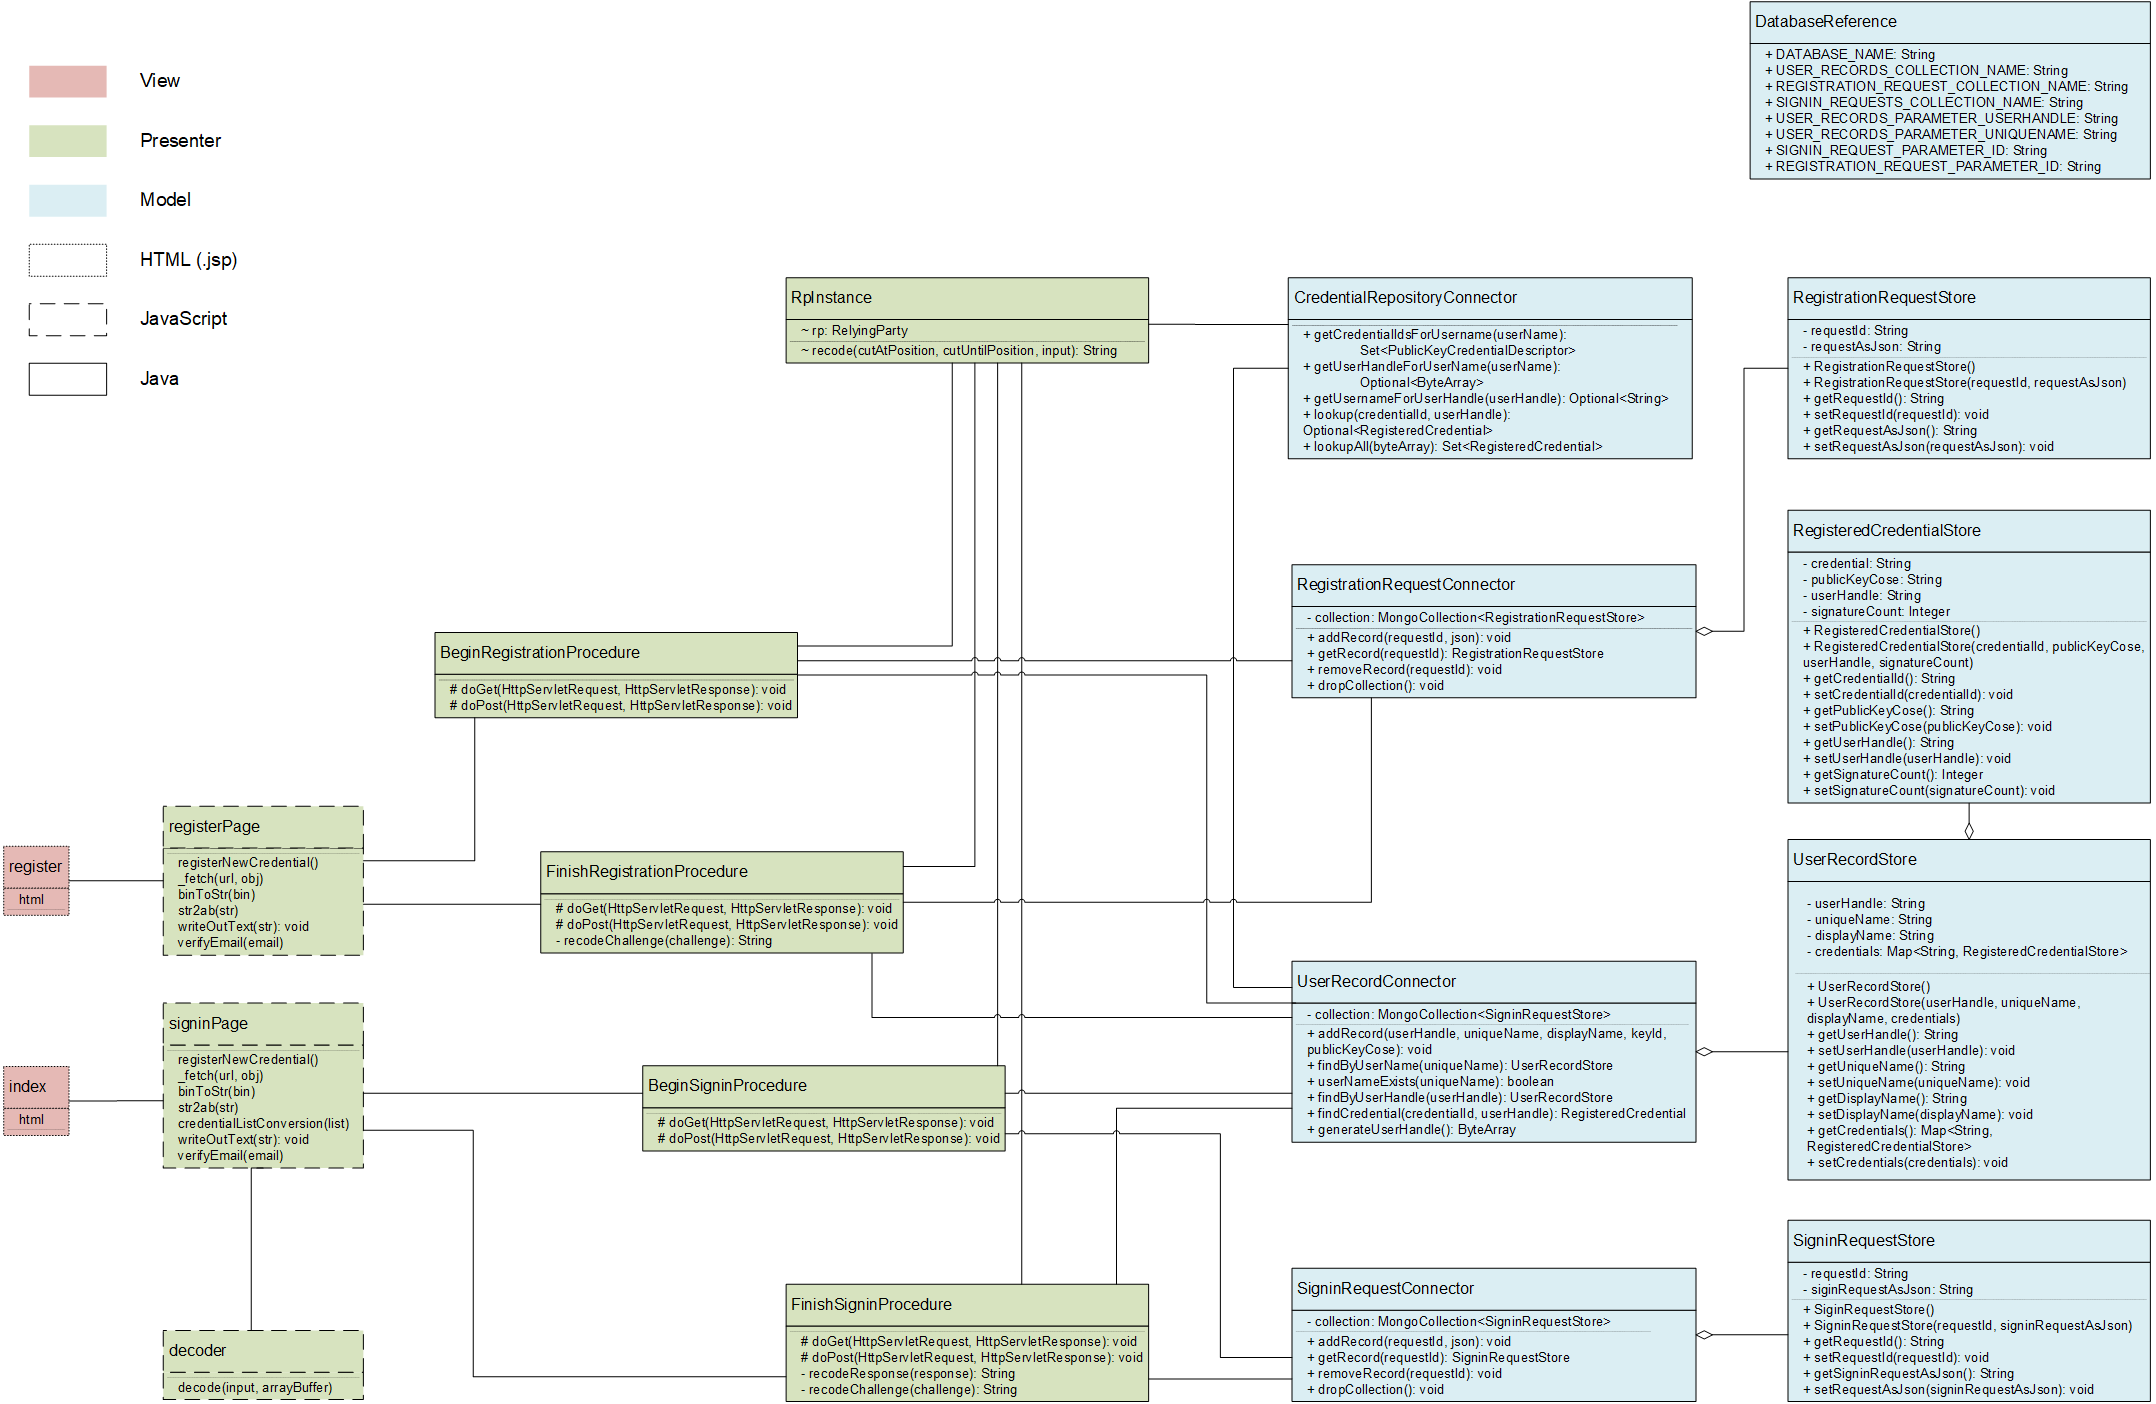
\includegraphics[width=\textwidth]{class-diagram}
    \caption{Class diagram for the authentication part of the prototype. The red colour represents the view pattern, the green colour represents the presenter and the blue colour represents the model.}
    \label{fig:class-diagram}
\end{sidewaysfigure}
\restoregeometry
    
\subsubsection{Flows}
The authenticator registration process corresponds to UC-5. The overview of the flow is as follows:
% 
\begin{enumerate}[noitemsep]
    \item A user-agent visits the specified endpoint of the \acrshort{aaserver}: \texttt{/AAFidoServer/register} and is served a static HTML page (class \texttt{register}) and a corresponding JavaScript file (class \texttt{registerPage}), which captures user's input.
    \item Once the user fills in the data and pushes the Register button, a \linebreak\texttt{/AAFidoServer/begin-registration} endpoint is contacted. In this endpoint a \linebreak\texttt{RegistrationRequest}, carrying the challenge and relevant relying party data is created, saved into database and sent in JSON format to the user agent.
    \item The user agent unwraps the JSON format and uses the included parameters to call \linebreak\texttt{navigator.credentials.create()} method, which is implemented by the browser and which prompts the user to use their authenticator. Figure~\ref{fig:key-prompts} shows the prompts displayed after the methods is called.
    \item If the user activates an authenticator, the browser returns an \linebreak\texttt{AuthenticatorAttestationResponse} object, containing initial information passed in the request, plaintext information about the newly created key pair such as credential ID and the public key, and the contents of the attestation response object signed over with the authenticator private key. The attestation response is passed by the JavaScript code to the \texttt{/AAFidoServer/finish-registration} endpoint on the \acrshort{aaserver}.
    \item The attestation response is processed and and compared with the \texttt{RegistrationRequest}, which is retrieved from the database. If the received response matches the original request, a user record is created in the database with user's `personal' details (unique name and display name) and relevant credential details, and the user is notified on the registration page.
\end{enumerate}

\begin{figure}[htb]
    \centering
    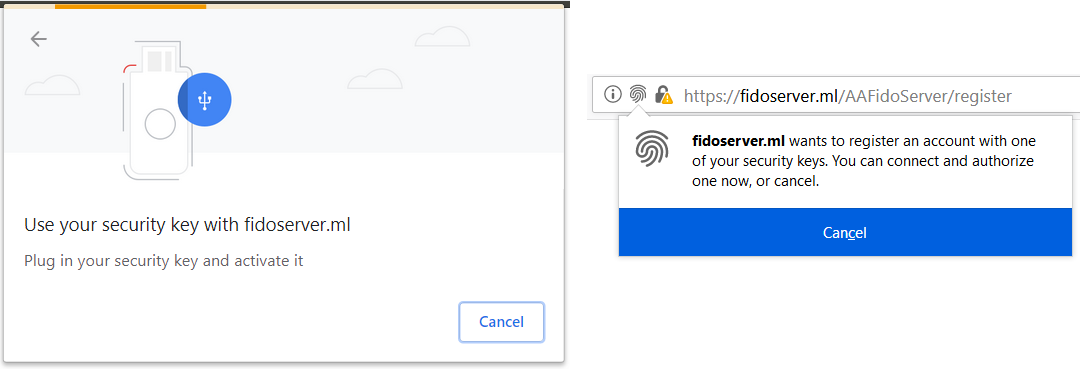
\includegraphics[width=.75\textwidth]{key-prompt}
    \caption{Propts to use an authenticator as displayed by the Chrome (left) and Firefox (right) browsers.}
    \label{fig:key-prompts}
\end{figure}

The sign-in process in this part of the prototype corresponds to steps 3 and 4 of UC-1 (see Table~\ref{tab:useCase_01} on page~\pageref{tab:useCase_01}). The detailed flow of the sign-in procedure is similar to the registration procedure described above. The server endpoints are replaced with the corresponding sign-in endpoints, \texttt{RegistrationRequest} is replaced with an \texttt{AssertionRequest} and the \texttt{AuthenticatorAttestationResponse} is replaced with an \texttt{AuthenticatorAssertionResponse}. When the \texttt{AssertionRequest} is created, a list of credentials associated with user's account is retrieved and included in the request. This list is presented to the authenticator during the \texttt{navigator.credentials.get()} method call. If the authenticator recognises a credential ID it previously created from the list, it produces an \texttt{AuthenticatorAssertionResponse} and the flow continues similarly to the registration flow.

\subsubsection{Testing}
Static testing was used to verify the correctness of the prototype flows. Code review was the main testing method, aided by automated code analysis. The testing verified the viability of the flow and identified several places, where more rigorous error handling was required. Debugging was also performed on small parts of the code, however the debugger could not be attached to the server and thus the debugging could not be used for the entire web application.
\subsection{OAuth \& OIDC and etc. NEW HEADING NEEDED} \label{sec:implementation-oauth}
% TODO heading ¯\_(ツ)_/¯

This section describes the implementation of OAuth and \acrshort{oidc} in our prototype. This part of the prototype implements two use cases: the \textit{UC-1 -- Sign-in}, where the basic user information are obtained using \acrshort{oidc}, and the \textit{UC-16 -- Access protected resources}, where the authorisation of the user is carried out and access to resources is granted or denied.

\subsubsection{Setup}
Various approaches to implementation of these use cases could have been adopted. Since we use \acrfull{gcp} to host the \acrshort{aaserver} in the Authentication flow, we also decided to use Google Cloud Compute Engine to carry out the rest of the Access Policy Enforcement flow. Therefore, initially, the \acrlong{gcp} was chosen for this scenario as well.

Google Cloud Community\footnote{\url{https://cloud.google.com/community}, accessed 19 May 2019} offers a compact guide for implementing OAuth2 on the \acrshort{gcp}, which we used to get understanding on how to implement it there~\cite{Awyu2018UnderstandingCloud}. Based on the guide we created a project on \acrshort{gcp} with client and user entities in the Datastore and Token, Auth, and Sign-in functions as described. Despite closely following the steps outlined in the guide, the solution did not achieve the desired results even after several modifications. The exact reason was not determined, but system logs indicated that recent changes to the \acrshort{gcp} Datastore\footnote{\url{https://cloud.google.com/datastore/release-notes\#august_22_2018}, accessed 20 May 2019}, broke the functionality described in the guide.
% , everything has been implemented as instructed, the server did not work and we did not manage to get over the error experienced, despite trying to implement our own solution based on the example. 
Therefore, we decided to move further and try different set-up and platform.

Looking for another approach to implementation of OAuth and \acrshort{oidc}, we found that Spring framework\footnote{\url{https://spring.io/}, accessed 19 May 2019} (together with Spring Boot\footnote{\url{https://spring.io/projects/spring-boot}, accessed 19 May 2019} and Spring OAuth\footnote{\url{https://spring.io/projects/spring-security-oauth}, accessed 19 May 2019}) could be used for this flow. Spring framework is an open source \acrshort{ioc} container and application framework which is written in Java for the Java platform. Spring Boot is used for development of spring applications without the need of deploying WAR files. It configures the application automatically based on dependencies as well as libraries if possible. Spring OAuth is a part of the Spring Security project, which enables easy implementation of OAuth2 using Spring models.

Several guides on the subject were followed, but many introduced errors because of incompatibility of newer versions of libraries they used. A guide by Federico Yankelevich~\cite{Yankelevich2016OAuth2Enterprises} was found to be suitable for our problem and was free of the incompatibility errors. The author defines: \textit{authorisation server}, \textit{resource server} and \textit{web application} in the guide. We implemented and configured this part of the prototype according to this guide and refer to it in the following sections.
% 
% Further in this section, we will explain the workings of this example and its flows. The code used and submitted with the report is the one from the example (available at~\cite{Yankelevich2016OAuth2Enterprises}), having minor changes made to it. 

In the application, three different clients are defined: account-admin, account-read, account-write, where each of them is having different access level to the resource, the \textit{message} which can be read or updated. Account-admin can both read and update the message, account-read can only read and account-write can only update the message. The application uses The Client Credential grant flow, which is used when the client application requires access to own resources and to obtain the access token.

\subsubsection{Flow}
To start the authorisation and resource servers, separate terminals have to be used and to deploy both servers locally on \texttt{localhost:8080} and \texttt{localhost:9090} respectively. Once started, there are two options for the client to access the resource:
% 
\begin{enumerate*}[label=(\roman*)]
    \item open another terminal and use \acrshort{curl} commands to communicate with servers, 
    \item starting the web application in another terminal and in the web browser access \texttt{localhost:9999} where the interface is available for reading and updating the message.
\end{enumerate*}

When accessing the resources using the first method, \acrshort{curl} command specifying the credentials of client, target resource and grant type is used, such as \texttt{curl account-admin:password -admin@localhost:8080/auth/oauth/token -d grant\_type=client\_credentials}. This way the \textit{access token} is obtained from the \textit{authorisation server} which first verifies client's credentials, then accesses the target resource and issues the \textit{access token}, which can be used for the message resource access, both read and update based on client's access level. The \textit{access token}'s validity is set to 90 seconds, during which the token can be used to manipulate the message resource while only contacting the \textit{resource server} to do so. Once the validity of the \textit{access token} has expired, the \textit{authorisation server} is contacted again to obtain fresh \textit{access token} which can then be used.

If second method is used, the same happens in the background, but instead of using commands in the terminal, user interface with text boxes and buttons is available to interact with in the web application. Also, the communication is ongoing between the web application and the \textit{resource server} instead of a terminal window and the \textit{resource server} as in previous method.

\bigskip \noindent
In the above explained implementation of UC-1 and UC-16, the \acrshort{oidc} is not implemented, while OAuth is implemented but not with an Authorisation grant flow as intended. Also, it is not the user who is signing-in to the service, its rather the client who is being verified and is accessing the resource. This way, we can see that the \acrshort{oidc} and OAuth part of the intended prototype has not been fully and successfully implemented, alternatively, Client Credentials Grant flow has been implemented to show how access token is obtained and used for resource access.

% Goal
% What was a goal to implement
% Implement UC-1 and UC-16 (generalisation of 17 and 18)

% Set-up
% different approaches, tutorials and libraries used
% give examples with links
% what were the struggles

% showcase the one chosen
% what are the entities being implemented
%     - authorisation server
%     - resource server
%     - web-app

% what is being used for implementation
%     - spring boot
%     - run in command/powershell

% what it does
%     - user credential flow
%     - give the client access token to access resources + scopes
%     - also refreshes the access token every 60s
%     - can read & write in web-app
%     - change scopes/privileges
%     - run as three local servers in terminals

In this chapter, the implementation of the prototype is described in two parts: Authentication and Authorisation. The setup, technologies and libraries are explained, followed by the overview of implemented system flows. Lastly, the testing methods are mentioned briefly. 

The Authentication part of the prototype is fully implemented, fulfilling the use cases and requirements set to be implemented. The second part, Authorisation, does not implement the use cases and requirements in full-scale, while it still demonstrates the flows and use of tokens in OAuth.